%Report of master graduation
%
% by Sylvain Blunier 
%
%main page for compilation

\documentclass[a4paper,11pt]{article}

%\usepackage{graphicx,epsfig,color,rotating}
\usepackage[dvips]{graphicx}% Include figure files
\usepackage{wrapfig}
\usepackage{xspace}
%\usepackage{dcolumn}% Align table columns on decimal point
%\usepackage{bm}% bold math
\usepackage[T1]{fontenc} % Encodage des caractères en sortie.
%\usepackage{textcomp} % Jeu de symboles complémentaires.
\usepackage[USenglish]{babel} % Support de la langue anglaise.
\usepackage{amsmath}
\usepackage{pstricks}
\usepackage{color}

\usepackage{hyperref}

\usepackage{enumitem}
\usepackage{pifont}

\usepackage{listings}

\definecolor{jaunecasse}{RGB}{255,255,153}

\lstset{
frame=single,
framerule=0pt,
language=bash,
basicstyle=\ttfamily\small, %
identifierstyle=\color{red}, %
keywordstyle=\color{blue}, %
stringstyle=\color{black!60}, %
commentstyle=\it\color{green!95!yellow!1}, %
columns=flexible, %
tabsize=2, %
extendedchars=true, %
showspaces=false, %
showstringspaces=false, %
%numbers=left, %
%numberstyle=\tiny, %
breaklines=true, %
breakautoindent=true, %
captionpos=b,
backgroundcolor=\color{jaunecasse}
}


%\usepackage[tikz]{bclogo}

%\usepackage{axodraw} 

\graphicspath{{Img/}}

\renewcommand{\arraystretch}{1.4}

%%%% debut macro %%%%
\newenvironment{changemargin}[2]{\begin{list}{}{%
\addtolength{\leftmargin}{#1}%
\addtolength{\textwidth}{#2}%
}\item }{\end{list}}
%%%% fin macro %%%%

\addtolength{\hoffset}{-1.5cm}
\addtolength{\textwidth}{3cm}

%\addtolength{\topmargin}{-.875in}

\addtolength{\textheight}{3cm}
\setcounter{secnumdepth}{5}

\begin{document}


\title{Report of CERN Internship} %\\ force le passage a la ligne

\author{Sylvain Blunier}

\maketitle
\section{Context}

\section{Objectives of the mission}

In ATLAS, users can access to the datas of the GRID via a protocol that might be changed, they have to import the files they need on their computer to be able to use it. We want to use the https protocol so that the user can access to the datas directly from where they are stored. This function is already developped and should be tested.\\

The first objective is to make a routine that can be executed on the sites which will make a test on some stored datas and check if the new function is working. The routine will have to access to datas, to be able to use them like making work a standard benchmark of data analize, and give some feedback about possible implementation mistakes and the performances of the protocol. Then we should be able to improve the new funcionality.\\


%Until now, the user access to their data via Webdav, that should be changed to Rucio

\section{Details of the implementation}


\subsection{Davix integration in ROOT}

The integration of Davix in ROOT was done on lxplus. Explanation are given to built root for cvmfs, the ROOT and Davix folders will be separated.\\

\subsubsection{Get Root}

In a folder where you will want to build your project, get the right version of ROOT:

\begin{lstlisting}
	> git clone http://root.cern.ch/git/root.git
\end{lstlisting}

To select the needed version, it is useful to know which one are available with:

\begin{lstlisting}
	> cd root
	> git tag -l
\end{lstlisting}

then to get the right version:

\begin{lstlisting}
	> git checkout v5-34-19
\end{lstlisting}

replacing "v5-34-19" by the version you want.


%%%%%%%%%%%%%%%%%%%%%%%%%%%%%%%%%%%%%%%%%%%%%%%%%%%%%%%%%%%%%%%%%%%%%%%%%%%%%%%%%%%%
\subsubsection{Get and compile Davix}

Out of the recent downloaded ROOT folder download git from the public repository (here we will give the commands assuming that davix/ and root/ are in the same directory):

\begin{lstlisting}
	> (cd ..)
	> git clone http://git.cern.ch/pub/davix
\end{lstlisting}

Just like we did for look at the version you want with:


\begin{lstlisting}
	> cd davix
	> git tag -l
\end{lstlisting}

and select the right version:


\begin{lstlisting}
	> git checkout R_0_3_4
\end{lstlisting}

Now we will build Davix, to do that you can follow the steps here or you can also look at \textit{README} where there are different ways to compile Davix, here we detail our way to compile Davix in embedded mode.


\begin{lstlisting}
	> mkdir -p build
	> git submodule update --recursive --init
	> cd build
	> cmake -D BOOST_EXTERNAL=NO -D CMAKE_INSTALL_PREFIX=/ ..
	> make
\end{lstlisting}

Now we will get the libraries to make possible integration in Root (still in the \textit{build} folder):


\begin{lstlisting}
	> mkdir -p root
	> make install DESTDIR=root/
\end{lstlisting}

Now you should have the libraries in davix/build/root/lib64/

%%%%%%%%%%%%%%%%%%%%%%%%%%%%%%%%%%%%%%%%%%%%%%%%%%%%%%%%%%%%%%%%%%%%%%%%%%%%%%%%%%
\subsubsection{Build ROOT}

The first step is to configure ROOT, then go first in your root folder and configure it with:

\begin{lstlisting}
	> (cd ../../../root)
	> ./configure --with-xrootd=/afs/cern.ch/sw/lcg/external/xrootd/3.2.7/x86_64-slc6-gcc48-opt --enable-davix --with-davix-incdir=../davix/include/davix/ --with-davix-libdir=../davix/build/root/lib64/
\end{lstlisting}

the first argument of \textit{configure} can be set only on cvmfs, if you only want root+davix without xrootd replace it by \textit{--disable-xrootd}. Make sure davix and xroot appear in the list of \textit{Enable support} that is printed at the end of the output of \textit{./configure}, obviously if you don't want to integrate xrootd it should be in the list.\\

Now compile root:

\begin{lstlisting}
	> make
\end{lstlisting}

Uncomment the two following lines in the file etc/system.rootrc:

\begin{lstlisting}
	709 Davix.GSI.CACheck: y
	717 Davix.GSI.GridMode: y
\end{lstlisting}

and finally, \underline{only if you don't want this version to be propagated on cvmfs} copy the compiled libraries of Davix in the lib folder of root:

\begin{lstlisting}
	> cd ..
	> cp davix/build/root/lib64/* root/lib/
\end{lstlisting}

Select the recent build patch with:

\begin{lstlisting}
	> source root/bin/thisroot.sh
\end{lstlisting}

%%%%%%%%%%%%%%%%%%%%%%%%%%%%%%%%%%%%%%%%%%%%%%%%%%%%%%%%%%%%%%%%%%%%%%%%%%%%%%%%%%%%

\subsubsection{Direct building from ROOT}

It is possible not to do the second part. Run the script \textit{installDavix.sh}:

\begin{lstlisting}
	> cd root/
	> ./build/installDavix.sh
\end{lstlisting}

It will download direclty Davix but you will have no choice on its version. You can also to that with xrootd in fact with \textit{installXrootd.sh}. The compilation of Davix will also have to be done separatly.

\subsection{Measuring the time to access datas}

We will see two type of histograms that give us informations about the flow of data transfer. But first let us explain how is working the code.\\

First get the url of a .root file you want to read, we will call it "http://url". The idea of the program is to open the file, select a tree \textit{"physics"} and read all the events of the branches \textit{"el\_n"} and \textit{"mu\_n"}. When an event is read we get the time from the beginning of reading and save it. When the branches are fully read, we create an histogram with the times we measured. This histogram has bins of 1 second and their value corresponds to the number of event read during this second.\\

The code is mainly divided in two functions:

\lstset{language=c++}
\begin{lstlisting}[frame=single,framerule=0pt]
	vector<int> fillTimes(char* fileName);
\end{lstlisting}

The takes in argument the url of the file, and return the vector of times. This funcion is the one that opens the file, select the branch we want to read, and finally read them saving the current time.\\


\begin{lstlisting}[frame=single,framerule=0pt]
	void createHistogram(vector<int> datas,char* nameFile, char* nameSite, char* nameProcessor);
\end{lstlisting}

takes in argument:

\begin{itemize}
	\item \textit{datas}: The times we got from \textit{fillTimes}
	\item \textit{nameFile}: The name of the .root file that will be generated
	\item \textit{nameSite}: Name of the site where we are reading (for the title)
	\item \textit{nameProcessor}: Name of the processor where it is running (for the title)
\end{itemize}

This function doesn't return anything because the outputs are generated where the file is. Finally the main function is:

\begin{lstlisting}
	int main(int argc, char* argv[])
	{
		vector<int> timeDatas;
		timeDatas = fillTimes(argv[1]);
		createHistogram(timeDatas,getFileName(argv[1]),getSite(argv[1]), argv[2]);
		return 0;
	}
\end{lstlisting}

where:

\begin{itemize}
	\item \textit{argv[1]} = "http://url"
	\item \textit{argv[2]} = Name of the processor
\end{itemize}

\textit{getFileName(string url)} extract the name of the file from "http://url" and \textit{getSite(string url)} extract the name of the site where we are reading from "http://url".\\

Figure ~\ref{fig:timeHistogram} shows an example of data access in function of the time, the program ran on lxplus and read at DESY\_ZN. In section ~\ref{sec:results} there are more histograms and comments on the results.\\

\begin{figure}
	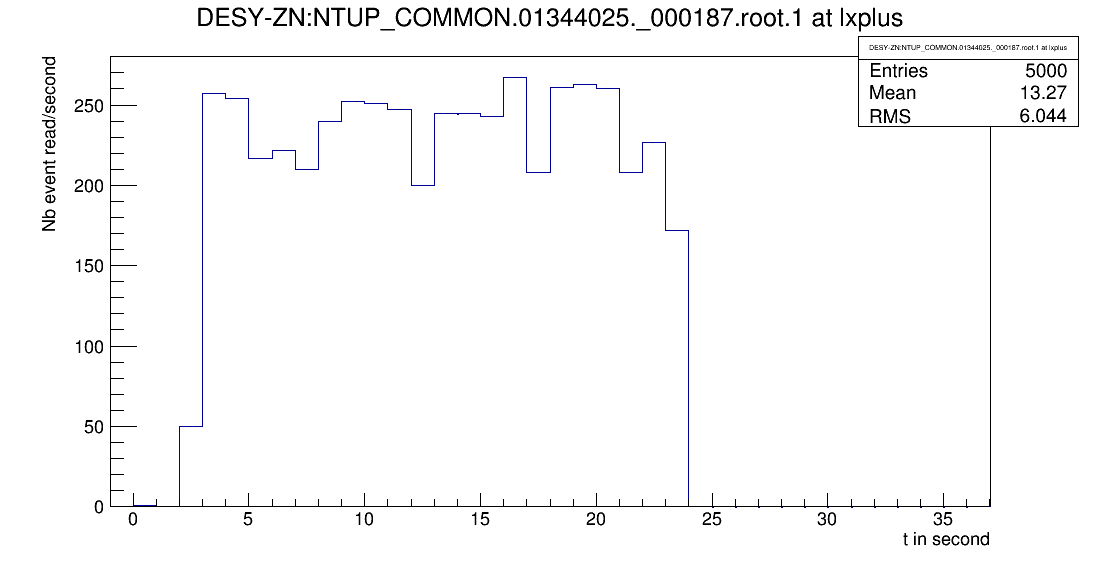
\includegraphics[width=1.1\textwidth]{timeHistogramDESYZN}
	\caption{Flow of Events read for each second at DESY\_ZN}
	\label{fig:timeHistogram}
\end{figure}


We can now see the evolution in the time of remote data access. But we have no idea of if we repeat the experiment the result will be the same, in other words we want to have some stastistics informations about the flow of datas. The idea is simply to repeat this experiment many times. To do that we will stop getting the time to each event reading but we will only get the time to get all datas, which corresponds to the last value of the vector in the previous case.\\

The functions are the same, with little differences:

\begin{itemize}
	\item \textit{fillTimes} will return only one \textit{int} which corresponds to the time to get all datas.\\
	\item \textit{createHistogram} will create an histogram only if none exists with the same processing site (where it runs) and the same read site. If this one already exists the function just open it and append the time divided by we just got. \\
\end{itemize}

This means that our histogram will not give evolution in time but the mean of events read per second, that will be called \textbf{events rate}. While we repeat the experiment the events rate of the file will be added to the histogram. In figure \ref{fig:eventsrateatDESYZNtoLRZ} the program was repeated 100 times, we can see a gaussian with a statistic error and a mean events rate.


\begin{figure}
	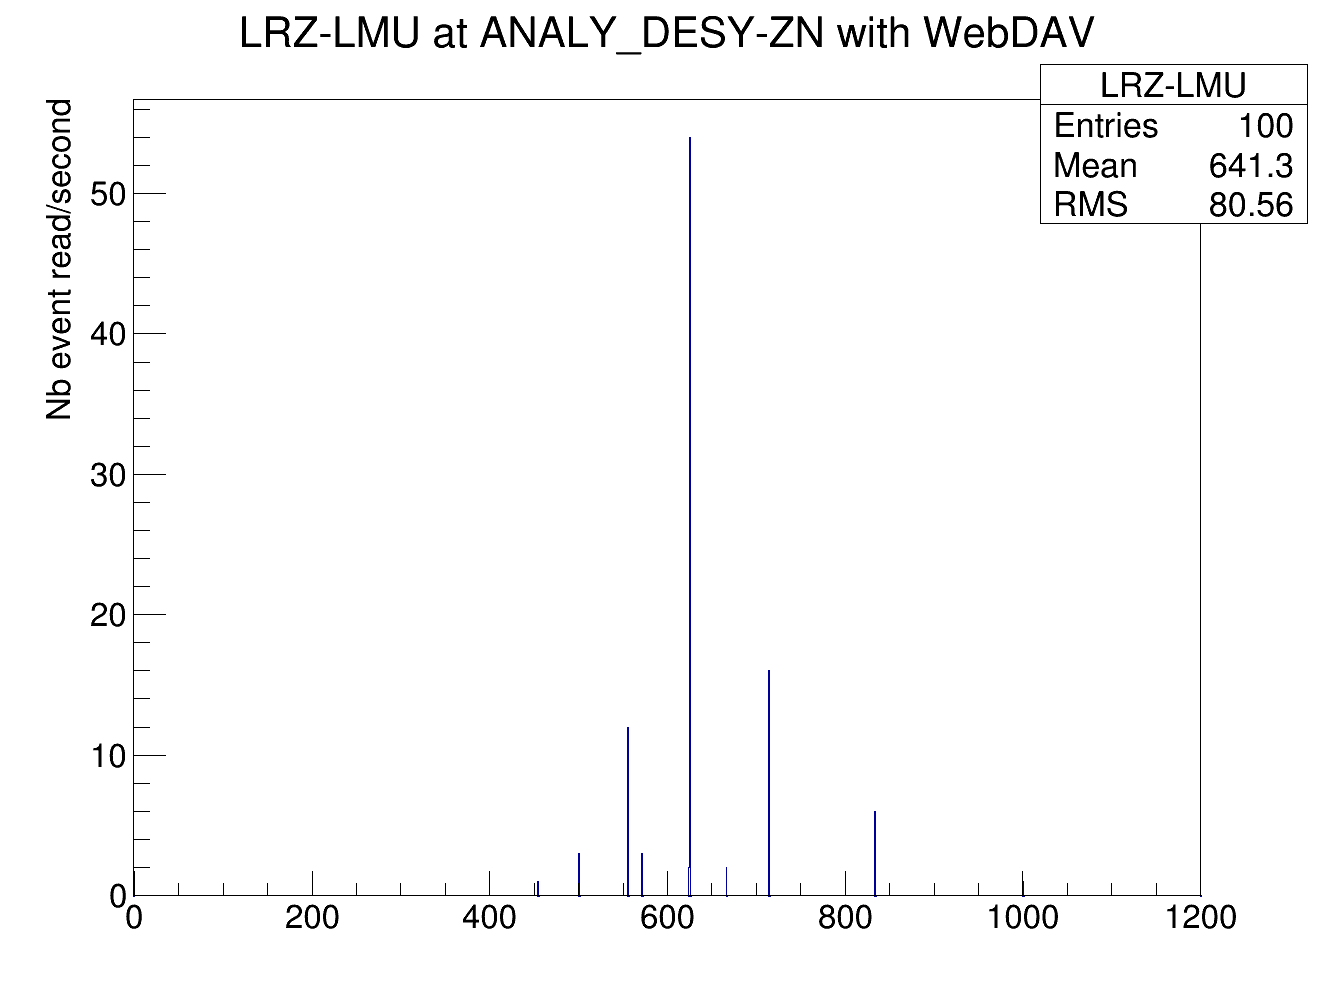
\includegraphics[width=1.1\textwidth]{eventsrateatDESYZNtoLRZ.png}
	\caption{100 events read at LRZ, processed at DESY} 
	\label{fig:eventsrateatDESYZNtoLRZ}
\end{figure}

\subsection{The jobs}

Until now we saw how to use Davix and how we want to analyse the events rates. But to do that it's also importante to understand how to send the jobs and to do that it's necessary to understand the command \textbf{prun}.

The more important to know about prun is how to use... the manual ! All the informations in this part are in th manual.

\lstset{language=bash}
\begin{lstlisting}
	prun --help
\end{lstlisting}

A CERN-twiki is also available as a tutorial where you can find more informations about what is prun:\\
\begin{center}
	\url{https://twiki.cern.ch/twiki/bin/view/PanDA/PandaRun}
\end{center}

In some words: \textit{"prun is a Panda-client software which allows users to submit general jobs to Panda"} (source: \url{https://twiki.cern.ch/twiki/bin/view/PanDA/PandaRun}). Here we will see how we used prun for our specific davix-jobs.\\

We will show an complete example, for that we asume we have a simple program \textit{main.C} that opens a file and read is as presented before but without any measurement. 

\begin{lstlisting}
prun --outDS user.sblunier.ariac001.ANALY_DESY-ZN --rootVer=5.34.19-davix_p1 --cmtConfig=x86_64-slc6-gcc48-opt --bexec make --exec "./main https://voatlasrucio-redirect-prod-01.cern.ch/redirect/mc12_8TeV/NTUP_COMMON.01272994._000002.root.1?rse=DESY-ZN_DATADISK nocache" --site=ANALY_DESY-ZN
\end{lstlisting}

The arguments means:

\begin{itemize}
	\item \textit{--outDS} user.sblunier.ariac001.ANALY\_DESY-ZN: name of the folder where we will be created the outputs of the jobs, it must begin by user.\textit{username} replacing \textit{username} by the correct name.
	\item \textit{--rootVer}=5.34.19-davix\_p1 design the root version you will use to run the job
	\item \textit{--cmtConfig}=x86\_64-slc6-gcc48-opt to design the correct compiled version
	\item \textit{--bexec} make: what will be run before the execution, here we just want to compile our program \textit{main.C}
	\item \textit{--exec} "./main https://voatlasrucio-redirect-prod-01.cern.ch/redirect/mc12\_8TeV/NTUP\_COMMON.01272994.\_000002.root.1?rse=DESY-ZN\_DATADISK nocache": command that will run the job, here \textit{main} with two arguments.
	\item \textit{--site}=ANALY\_DESY-ZN: To ask the job to be ran where we want
\end{itemize}

Note that this command could be much simpler, many of those arguments have default values but here we need to fix those parameters.\\

There are other parameters that will be used in the monitoring (see section \ref{sec:monitoring}):

\begin{itemize}
	\item \textit{--extFile}=proxy: We can send an external file with the job, here we need the proxy to allow remote access from the processing site.
	\item \textit{--outputs}=rootfile.root: File generated by the job that we will need to recover.
\end{itemize}

\subsection{The monitoring}
\label{sec:monitoring}

The idea of a monitoring started with the necessity to make a report of the status of WebDAV/https over the grid. We needed to know which are the sites that are working fine with Davix, and have some details of the problem for those where data remote access was not working. Inicially, this report was generated in pdf, this is still the case but finally it could be provided at webpage:\\
\url{http://sblunier.web.cern.ch/sblunier/webdavGridStatus/}\\

This monitoring is updated every day.

\subsubsection{Structure of the monitoring}
The monitoring is divided in three parts:\\

\indent	\textbf{A. \underline{Local tests:}} two tests per sites are done on lxplus: first with curl and second with davix.\\
Before giving the results of the tests some more informations are given: the type of storage the version of the tested site, the file that will be tested and the date and hour of the tests.\\
The curl command is trying to reach the file, rucio redirects the url on the headnode of the site and the site is in charge to locate the file on the right disk. This is what is done on this test, if the file is not found the relevant error of curl is reported.\\
The second test try to open and read one branch of this file using Davix and reports if this could be done successfully.\\
All of those tests are used to create the plots thta appear in introduction that give more general statistics. First, there are two pie charts that give the proportions of tests that worked fine and the proportion per error and finally a plot giving the number of sites that where successfull per day.\\

\indent	\textbf{B. \underline{The WebDAV events rate:}} Compilation of the results that ran over the grid.\\
Each day, one job is sent on each ATLAS site that has a Datadisk. This job creates a list of one file per Datadisk of the same cloud. A routine is sent for each file that opens the file, read one branch measure the time needed to complete the reading part and sent this time in an Histogram. This operation is repeated 100 times, and creates one histogram per Datadisk of the cloud. This means that each histogram should contain 100 entries. That's not always the case since sometimes no file is found, if the file is found but could not be opened or read the bin 0 is incremented. All the histograms are saved in a root file and this file is the output of the job.\\

Those jobs are in fact sent three times with three different configuration:
	\begin{itemize}
		\item \textbf{configuration 1:} Davix access, TTreeCache disabled
		\item \textbf{configuration 2:} Davix access, TTreeCache enabled
		\item \textbf{configuration 3:} xrootd access, TTreeCache enabled
	\end{itemize}

We download the results about 18 hours before sending it. In this part there are 7 histograms. The first three histograms give the number of file that could be read for each jobs configuration. In fact this corresponds to the number of all entries of the histograms from the outputs that are different from zero. A column corresponds to the output of one job, each cell to one histogram from the outputs. The histograms 4, 5 and 6 give the mean of the time of events rate for each Datadisk and the error.
The last histogram makes a direct comparison between the histograms 5 and 6: it represend the ratio (Davix events rate)/(xrootd event rates). If the result is above one Davix access is faster if not xrootd is faster.\\

\indent	\textbf{C. \underline{The jobs on the queues:}} Statistics about the jobs that ran for the previous part.\\
This part gives the status of the jobs for each configuration after the tests. Three status are possible: done (the job complete successfully), running (the job is running or has not been started), failed (crash of the job). A pie chart compile the proportion per status of the jobs.

\subsubsection{Technical details}

In this part we will explain in details how the monitoring is generated. The inicial idea of all of this work was only to make the first part in a pdf and became gradually bigger, it was not thought to give the other part so the code might not be easy to read. Nevertheless, at the end some effort was done to make it more ergonomic for the developer and hopefully can be read, maintained and even improved by some else. \\

The different languages used for this monitoring are C++, python, bash script, latex and html, however no html knowing is needed to purchase this work because it is directly generated by compiling latex. \\

The main folder is \textit{WebDAVMonitor} it contains 4 folders has shown in figure \ref{fig:WebDAVMonitor}. We will detail all of those parts.\\

\begin{figure}
	\center
	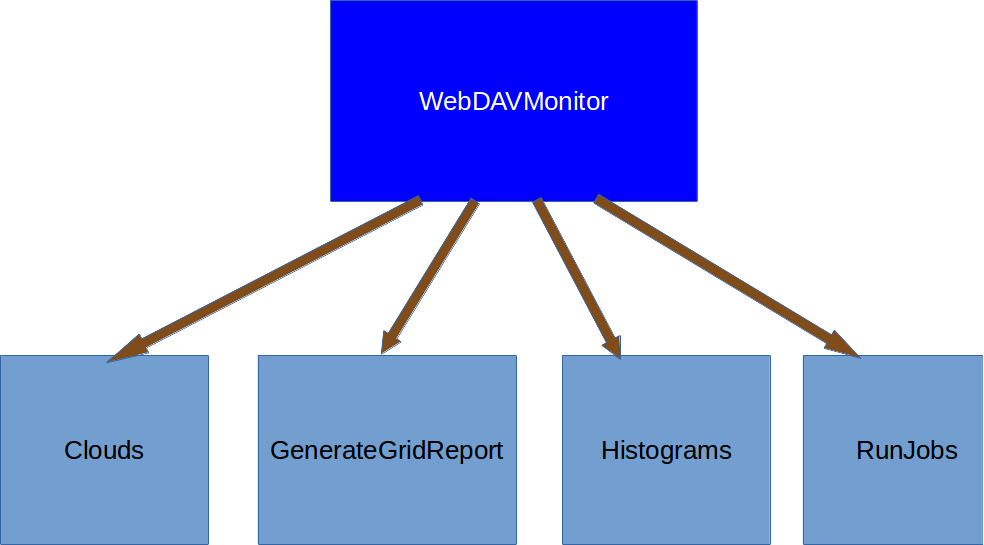
\includegraphics[width=0.7\textwidth]{WebDAVMonitor}
	\caption{Structure of WebDAVMonitor}
	\label{fig:WebDAVMonitor}
\end{figure}

\indent \textbf{A. \underline{Clouds:}}\\

\begin{figure}
	\center
	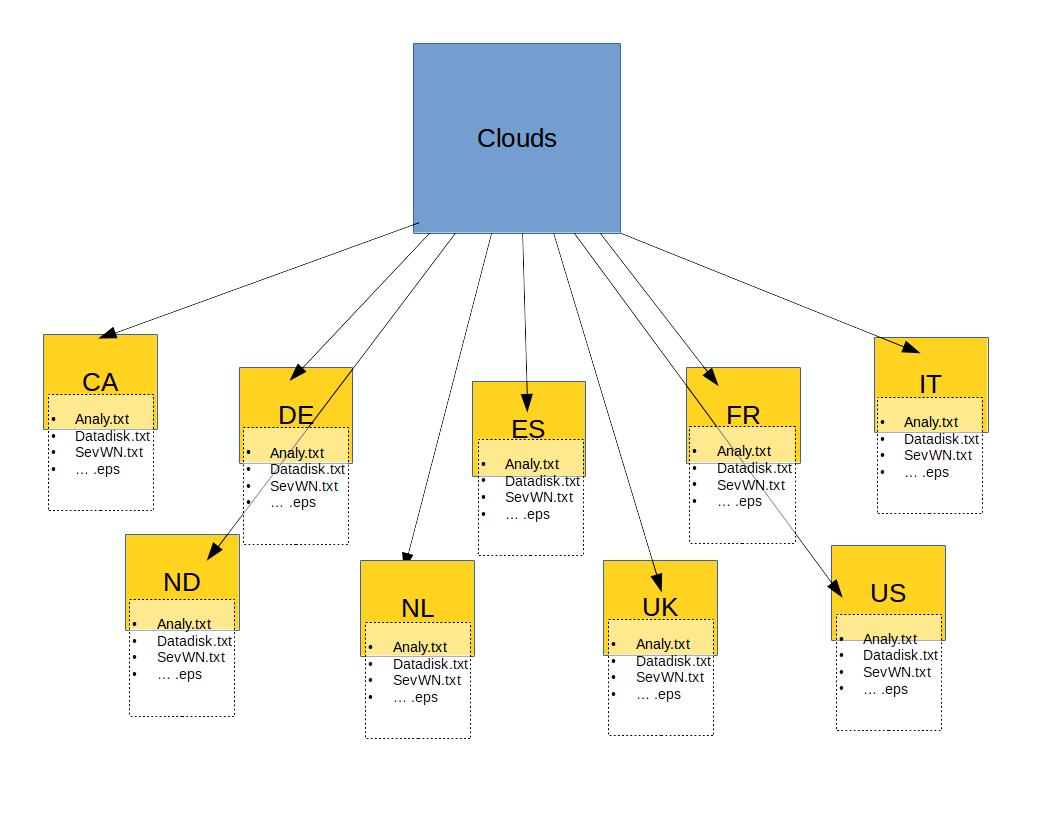
\includegraphics[width=0.8\textwidth]{Clouds}
	\caption{Structure of Clouds}
	\label{fig:Clouds}
\end{figure}

The folder \textit{Clouds} contains one folder per cloud, and each folder contains three files essential to the working of the monitoring:
\begin{itemize}
	\item \textit{Analy.txt:} contains the list of all the queues where we want to run the job on the cloud. This file will be read several times by the bash scripts that we will see later.
	\item \textit{Datadisk.txt:} like for the previous one, this file contains all Datadisks of the cloud, it's an exhaustive list.
	\item \textit{SEvsWN.txt:} to make the link between the disk and the queue that belong to the same cloud, will be used for the creation of matrix in part B of the monitoring.
\end{itemize}

The other files in those folder are file that are modified at each generation of the monitoring, they can be removed because they are not essential since they are created by the scripts:

\begin{itemize}
	\item \textit{PerCentFile.eps:} Histogram 1 of the monitoring, percent of file that could be read with configuration 1.
	\item \textit{tPerCentFile.eps:} Histogram 2 of the monitoring, percent of file that could be read with configuration 2.
	\item \textit{xPerCentFile.eps:} Histogram 3 of the monitoring, percent of file that could be read with configuration 3.
	\item \textit{EventRate.eps:} Histogram 4 of the monitoring, events rate with configuration 1.
	\item \textit{tEventRate.eps:} Histogram 5 of the monitoring, events rate with configuration 2.
	\item \textit{xEventRate.eps:} Histogram 6 of the monitoring, events rate with configuration 3.
	\item \textit{xRatio.eps:} Histogram 7 of the monitoring, ratio of common part of histogram 5 and 6.
	\item \textit{prun.txt:} prun commands that ran for the corresponding cloud, all the jobs are listed here, when a job is sent one line is written in this file. It's just an information file.
\end{itemize}

All the \textit{.eps} files are used to generate the monitoring, in fact when generating the latex the images are referenced directly in those folder.\\

\indent \textbf{B. \underline{RunJobs:}}\\

The rule of this folder is to send the jobs. It only contains files and this time most of them are essential. The general idea is to send one job per queue that will read 100 times one file per Datadisk of the cloud just as explained in the previous part. The jobs are labeled by a name of the type:
\begin{center}
	\textit{user.sblunier.?1allgrid????2.??3.ANALY\_?4}\\
\end{center}
where:
\begin{itemize}
	\item ?1 = m,t or x depending of the jobs configuration
	\item ????2 = number of the job, is incremented each day
	\item ??3 = name of the cloud
	\item ANALY\_?4 = site where the job is running
\end{itemize}
By doing that we guarantee that each job will have a different name (unless we reach ????2=9999)\\

\noindent \textbf{\textit{- main.C:}}
\textbf{Arguments:}\\
\begin{itemize}
	\item argv1: string, url of the file we are going to read
	\item argv2: string, name of the output file which will contain all the histograms.
	\item argv3: string, \textit{"ttreecache"} will activate TTreeCache while reading the file, something else disabled TTreeCache, there is no default argument
\end{itemize}

The output will be a file \textit{argv2.root} that contains the histograms. If the file exists the program will just append the bin to the histogram, else it creates it and append the measured value.\\

\noindent \textbf{\textit{- Makefile, main.o, main:}} For the compilation and executable of \textit{main.C}\\

\noindent \textbf{\textit{- listFilePeroSite.txt:}} Contains the list of file that will be read by \textit{main}. The url of the file is different depending on which protocol we want to use.\\
\noindent \textbf{\textit{- ttreeCacheBlackList.txt:}} When writing this report the root version used is 5.34.19-davix\_p1-x86\_64-slc6-gcc48-opt, with this version we get problems with some sites while using TTreeCache which make crash the jobs, this file contains the list of those sites. Nothing generates this file, it's purely based on testing the sites one by one.\\

\noindent \textbf{\textit{- launchJobs.sh:}} Read \textit{listFilePeroSite.txt:} and use it as argument to launch \textit{main} on each of the urls listed in.
\textbf{Arguments:}\\
\begin{itemize}
	\item arg1 = argv2 of main (\textit{ANALY\_SITE})
	\item arg2 = argv3 of main (\textit{"ttreecache"} or not)
\end{itemize}

If TTreeCache is enabled, the program checks if the site where the file is stored belongs to \textit{ttreeCacheBlackList.txt:}, if yes we look at the next one, else we process it normally.\\

\noindent \textbf{\textit{- getFiles.py:}} Python file that uses dq2 to pick some \textit{NTUP\_COMMON} files on the grid and store the url in \textit{- listFilePeroSite.txt:}. In the case of xrootd there is a list of endpoint corresponding to the site so that the file is able to create the url for xrootd. For WebDAV we use the general pattern of Rucio: \textit{"https://voatlasrucio-redirect-prod-01.cern.ch/redirect/"}.\\
\textbf{Arguments:}\\
\begin{itemize}
	\item sys.argv[1] = \textbf{"Davix"} or \textbf{"xrootd"} for the protocol needed
\end{itemize}

\noindent \textbf{\textit{- main.sh:}}

\textbf{Arguments:}\\
\begin{itemize}
	\item \$1: Cloud where the job is going to run
	\item \$2: argv2 of main (\textit{ANALY\_SITE})
	\item \$3: argv3 of main (\textit{"ttreecache"} or not)
	\item \$4: \textit{"davix"} or \textit{"xrootd"} depending on the protocol you want to use, argument necesarry to generate the right type of URL.
\end{itemize}

This script copies the file \textit{Datadisk.txt} in the local folder from the cloud corresponding to argument 2, run \textit{getFiles.py} using \textit{Datadisk.txt} and run \textit{launchJobs.sh}.\\

\noindent \textbf{\textit{- x509up\_u}xxxxx:} Valid proxy that will be needed for remote access, this file is sent with the job.\\

\noindent \textbf{\textit{- prun.txt:}} Output of the prun command executed by the script \textit{runPrun.sh}, information file.\\

\noindent \textbf{\textit{- runPrun.sh:}} The main function of this script is to execute the prun command to send the jobs. It also creates the files \textit{mjobIDs.txt}, \textit{tjobIDs.txt} and \textit{xjobIDs.txt} that will contain the number of the jobs by scanning the output of the prun command. This script activate the ATLAS commands (setupATLAS) activates Panda and dq2. It also select the root and Davix versions, copies the proxy from /tmp/.
It loops overall the folder of \textit{Clouds} and overall the items in \textit{Analy.txt} of the cloud, by doing that we send one job per queue giving the name of the output folder\\

\textbf{Arguments:}\\
\begin{itemize}
	\item \$1 = Cloud where you want the jobs to be sent, "all" for all the grid
	\item \$2 = number of the experiment, will be the number that labels the job serie (????2)
	\item \$3 = "ttreecache" or not
	\item \$4 = "davix" or "xrootd"
\end{itemize}

\begin{figure}
	\center
	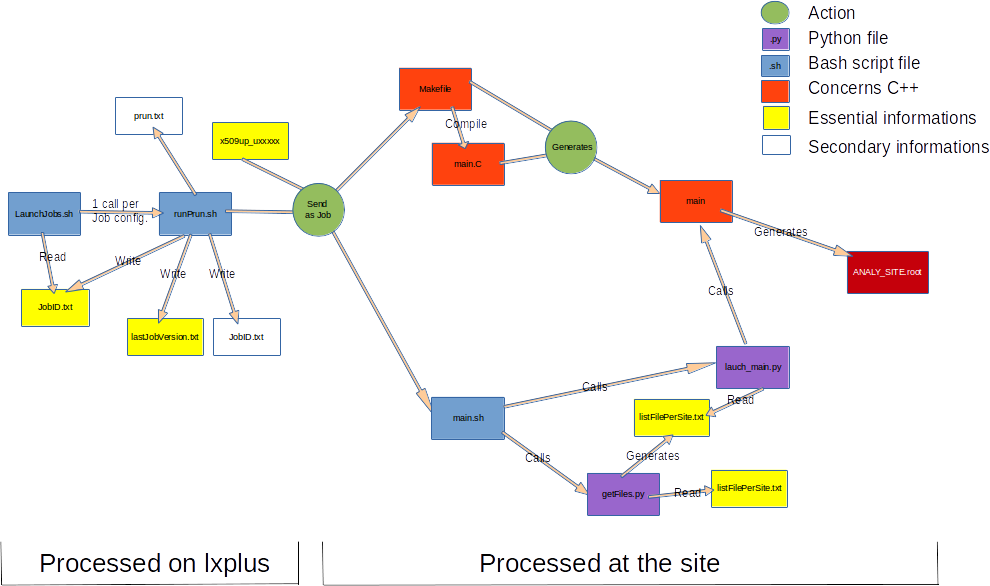
\includegraphics[width=1.1\textwidth]{runJobs}
	\caption{Block diagram of RunJobs}
	\label{fig:runJobs}
\end{figure}

Figure \ref{fig:runJobs} gives an overview of the working of all those files together.\\

\indent \textbf{C. \underline{Histograms:}}\\

The function of this folder is to contain the output of the jobs, meaning the \textit{.root} files.

\begin{figure}
	\center
	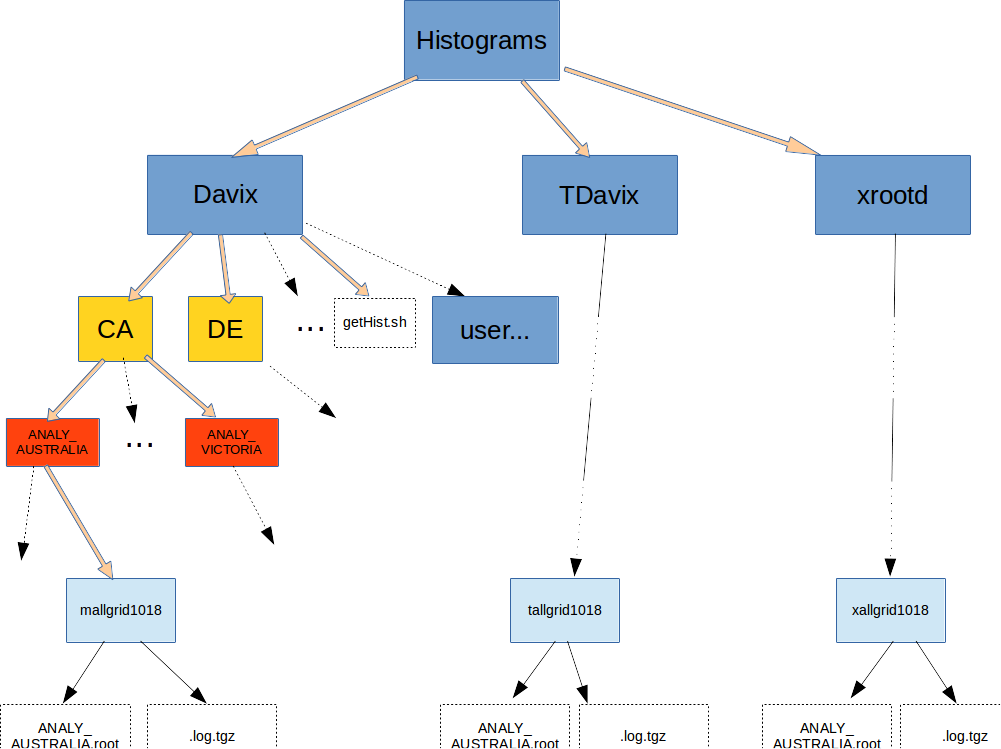
\includegraphics[width=0.7\textwidth]{histograms}
	\caption{Structure of Histograms folder}
	\label{fig:histograms}
\end{figure}

As shown in figure \ref{fig:histograms} the \textit{Histograms} folder contains three folders:

\begin{itemize}
	\item \textit{Davix}: Outputs of the first job configuration (TTreeCache disabled, Davix)
	\item \textit{TDavix}: Outputs of the second job configuration (TTreeCache enabled, Davix)
	\item \textit{xrootd}: Outputs of the third job configuration (TTreeCache enabled, xrootd)
\end{itemize}

They all have exactly the same structure, that's why we will only concentrate on the first one. The following depth contains folders named by the clouds, the clouds contains folders named by the queues where the jobs are ran. The queues folders contain folders that are called by the name of the corresponding experiment. This last folder is the one which will contain the outputs of the jobs: the \textit{.root} output and the logs.\\
This structure might be a little complicated but the goodness is that all the jobs are saved and we can at any moment have the details of a special result.\\
There might be others folder in \textit{Davix} that have the name of the jobs, they just are the outputs of the last downloaded job. \\

\indent \textit{\textbf{- getHist.sh:}} This script is here to distribute the outputs in their corresponding folders to keep them. It iterates over all the lines of the file \textit{clouds.txt} which is an essential file.\\


\indent \textbf{D. \underline{GenerateGridReport:}}\\

This part is the one which will write the latex report. It's divided in two sections, the first section treat all that requires dq2 and the second one generally needs root. This had to be separated because dq2 and root started to be incompatible during April 2014, this is not going to be fixed since dq2 is going to be replaced by Rucio.\\

Let us give an overview of those two parts before going into the details:

\begin{itemize}
	\item \textit{dq2Infos}: This part download and save the output of the jobs, generates one list of file url per cloud, and collect the versions of storage of the sites.
	\item \textit{writeLatex}: Generate the first part by testing curl and Davix locally, compile, creates, save the histograms and integrate them in the latex of part two and finally generate the part three by reading the html of the jobs on JEDI.
\end{itemize}


\begin{figure}
	\center
	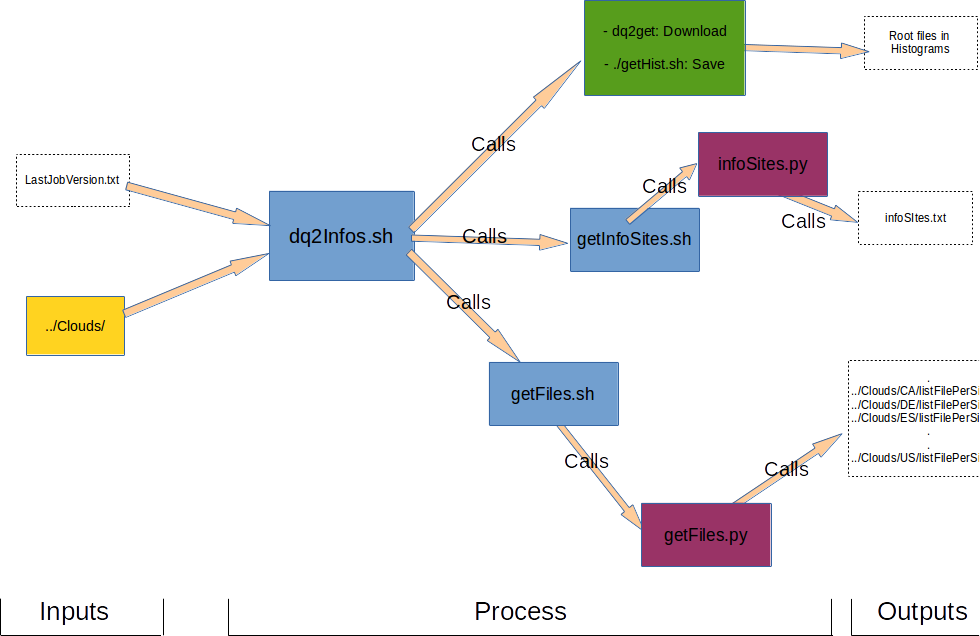
\includegraphics[width=0.9\textwidth]{dq2Infos}
	\caption{Functionning of \textit{dq2Infos.sh}}
	\label{fig:dq2Infos}
\end{figure}

In figure \ref{fig:dq2Infos} you can see how the first part is working, all the outputs will be necessary to produce the report with \textit{writeLatex.sh}, and in figure \ref{fig:writeLatex} the diagram for writeLatex which gives and overview on the last steps of the monitoring generation.


\begin{figure}
	\center
	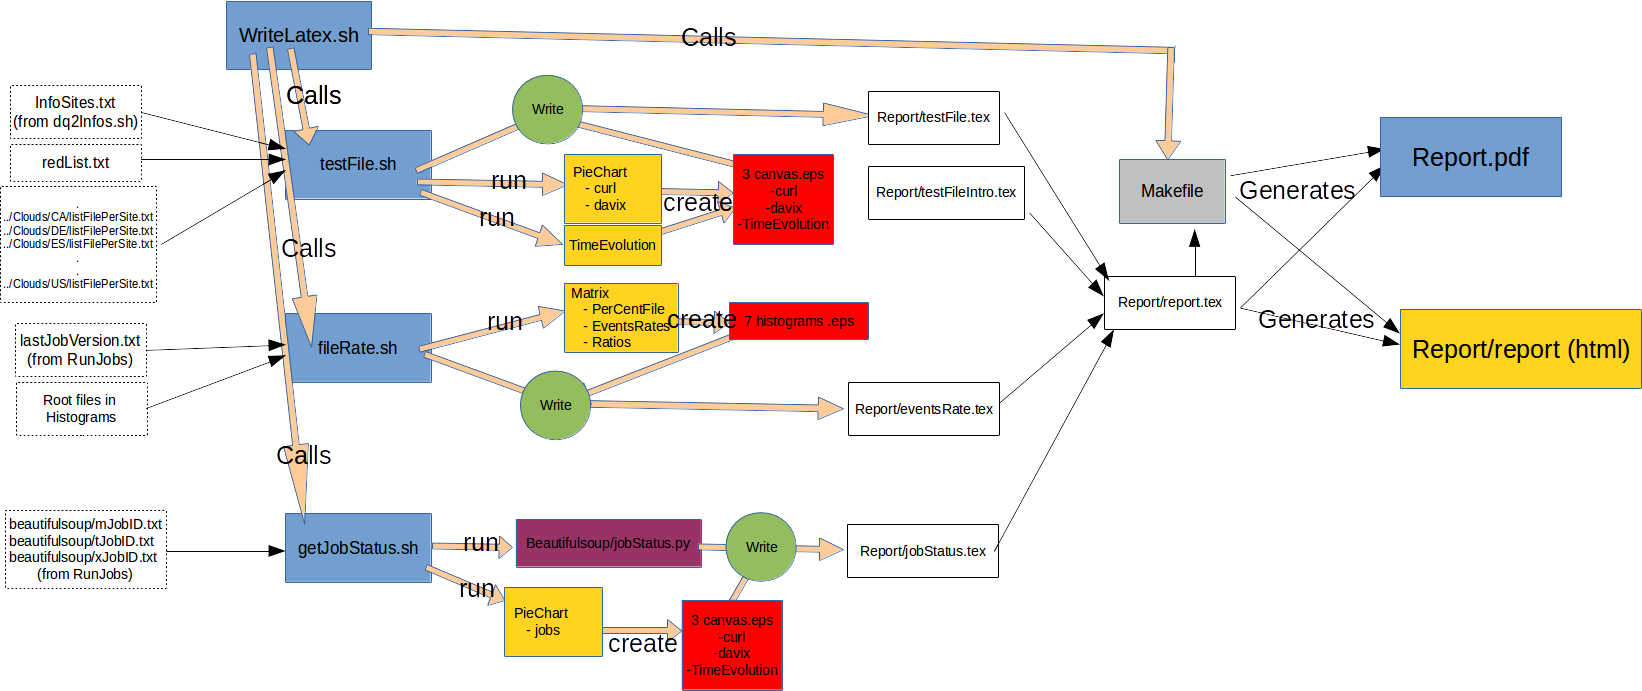
\includegraphics[width=1.1\textwidth]{writeLatex}
	\caption{Functionning of \textit{writeLatex.sh}}
	\label{fig:writeLatex}
\end{figure}

\section{Results of performances}
\label{sec:results}


\section{Improvements for the future}


\end{document}
%
% ****** End of file report.tex ******
